\documentclass[tikz,border=8pt]{standalone}
% Shared look for every TikZ diagram. Load with \input{../../tools/tikz-style.tex}
\usepackage[T1]{fontenc}
\usepackage{lmodern}
\renewcommand{\sfdefault}{lmr}  % diagrams use the same serif as the text
\usetikzlibrary{arrows.meta, positioning, shapes.geometric, calc, fit, backgrounds}
\definecolor{cblue}{HTML}{4C78A8}
\definecolor{corange}{HTML}{F58518}
\definecolor{cgreen}{HTML}{54A24B}
\definecolor{cred}{HTML}{E45756}
\definecolor{cpurple}{HTML}{B279A2}
\definecolor{cgrey}{HTML}{6B6B6B}
\tikzset{
  every picture/.style={font=\sffamily, line width=1.2pt},
  box/.style={draw=#1, fill=#1!12, rounded corners=4pt, align=center, inner sep=7pt, minimum height=1.1cm},
  box/.default=cgrey,
  arrow/.style={-{Stealth[length=3mm]}, draw=cgrey, line width=1.4pt},
  title/.style={font=\sffamily\bfseries\Large},
  note/.style={font=\sffamily\small, text=cgrey, align=center},
}
\AtBeginDocument{\hyphenpenalty=10000 \exhyphenpenalty=10000}

\begin{document}
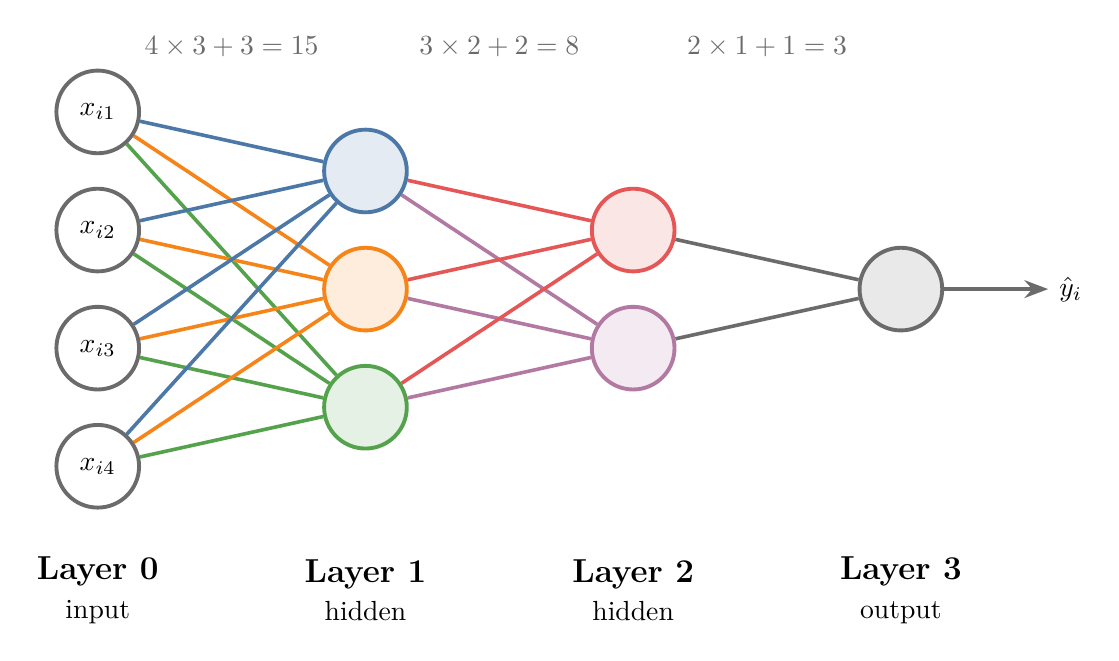
\begin{tikzpicture}[x=3.4cm, y=1.5cm,
  neuron/.style={circle, draw=#1, fill=#1!15, minimum size=1.05cm, line width=1.4pt},
  inp/.style={circle, draw=cgrey, fill=white, minimum size=1.05cm, line width=1.4pt}]
  % layer 0: 4 inputs
  \foreach \i in {1,...,4} \node[inp] (a\i) at (0, 2.5-\i) {$x_{i\i}$};
  % layer 1: 3 nodes, one colour each
  \foreach \j/\c in {1/cblue,2/corange,3/cgreen} \node[neuron=\c] (b\j) at (1, 2-\j) {};
  % layer 2
  \foreach \j/\c in {1/cred,2/cpurple} \node[neuron=\c] (c\j) at (2, 1.5-\j) {};
  % layer 3
  \node[neuron=cgrey] (d1) at (3, 0) {};
  \begin{scope}[on background layer]
  \foreach \i in {1,...,4} \foreach \j/\c in {1/cblue,2/corange,3/cgreen} \draw[\c, line width=1.3pt] (a\i) -- (b\j);
  \foreach \i in {1,2,3} \foreach \j/\c in {1/cred,2/cpurple} \draw[\c, line width=1.3pt] (b\i) -- (c\j);
  \foreach \i in {1,2} \draw[cgrey, line width=1.3pt] (c\i) -- (d1);
  \end{scope}
  \draw[arrow] (d1) -- ++(0.55,0) node[right] {$\hat{y}_i$};
  % layer labels
  \foreach \x/\t/\s in {0/Layer 0/input, 1/Layer 1/hidden, 2/Layer 2/hidden, 3/Layer 3/output}
    \node[align=center, font=\sffamily\large] at (\x, -2.55) {\textbf{\t}\\{\normalsize \s}};
  % parameter counts
  \foreach \x/\t in {0.5/{$4\times3 + 3 = 15$}, 1.5/{$3\times2 + 2 = 8$}, 2.5/{$2\times1 + 1 = 3$}}
    \node[note, font=\sffamily\normalsize] at (\x, 2.05) {\t};
\end{tikzpicture}
\end{document}
